\documentclass[crop,tikz]{standalone}
\usetikzlibrary{positioning,arrows,fit,calc}
\pgfdeclarelayer{bg}
\pgfsetlayers{bg,main}
\tikzset{
	>=stealth'
}
\begin{document}
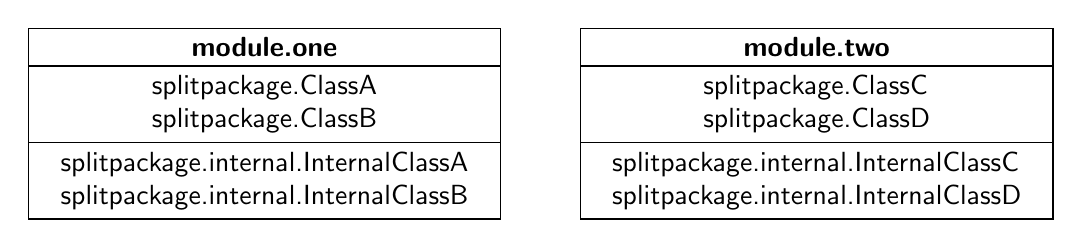
\begin{tikzpicture}[
node distance = 0mm,
every node/.style = {
	font = \sffamily
},
jar/.style = {
	draw,
	minimum height = 2.cm
},
package/.style = {
	draw,
	minimum height = 1.3cm,
	minimum width = 1.5cm
},
class/.style = {
	draw,
	fill = white,
	minimum height = \baselineskip,
	minimum width = .5cm
}
]

\node (module1title) [draw, font=\bfseries\sffamily, minimum width=6cm] {module.one};
\node (module1a) [draw, align=left, below = -0.1mm of module1title, minimum width=6cm] {splitpackage.ClassA\\ splitpackage.ClassB};
\node (module1b) [draw, align=left, below = -0.1mm of module1a, minimum width=6cm] {splitpackage.internal.InternalClassA\\ splitpackage.internal.InternalClassB};


\node (module2title) [draw, font=\bfseries\sffamily, minimum width=6cm, right = 1cm of module1title] {module.two};
\node (module2a) [draw, align=left, below = -0.1mm of module2title, minimum width=6cm] {splitpackage.ClassC\\ splitpackage.ClassD};
\node (module2b) [draw, align=left, below = -0.1mm of module2a, minimum width=6cm] {splitpackage.internal.InternalClassC\\ splitpackage.internal.InternalClassD};

\end{tikzpicture}

\end{document}